\section{Hardware}
As decided in \cref{systemArchitecture}, the system should consist of 2 subsystems: a sensor/actuator subsystem and a artificial intelligence subsystem. \sinote{Dette er under antagelse af at vi har valgt arkitekturen der sender regler til sensor subsystem}. This section will summarise the hardware requirements for the 2 subsystems.

\subsection{Sensor/actuator Subsystem}
The sensor/actuator subsystem consists of sensors, actuators and computational devices driving the sensors and actuators. The requirements for the sensors are elicited in \cref{}\sinote{mangler reference til hvor vi opstiller krav til sensorer/aktuation}. The requirements and a discussion these is listed below.

The hardware requirements for the sensor/actuator subsystem is:

\begin{itemize}
\item Analog and digital input/output pins should be accessible. This is required for connecting sensors and actuators to the boards controlling the sensor/actuator subsystem.
\end{itemize}

krav fra arkitektur
2 delsystemer:

sensor/aktuator:
in/out ben skal være tilgængelige
hukommelse for regler
ikke så kraftige
mulighed for real-time schedulering

krav fra analyse/specifikation
fysisk størrelse - lille
billig
ikke meget strøm





\subsection{Hardware on the Market}
The market has a variety of hardware to offer. These hardware include microcontrollers, that is programmable boards, as well separate modules for the micro controllers. The microcontrollers comes in variety of sizes, shapes, power consumption and computational capabilities.
\\\\
Even though the market is has much to offer, few of the microcontrollers are chosen because of their ability to suit this type of project. These micro-controllers are  considered based on the requirements mentioned in section\ref{sec:specification}.
\\\\The list of the hardware taken into consideration are following:
\begin{enumerate}
  \item Raspberry pi
  \item BeagleBone
  \item Arduino
  \item Teensy
\end{enumerate}
\subsubsection{Raspberry pi}
The raspberry pi is more than just a microcontroller. Rapsberry pi is a credit-card sized computer that runs linux operating system and can be plugged into a computer monitor or a TV. The devices uses a mouse and keyboard as I/O. The device is however programmable and thereby a candidate for embedded hardware. It is small but the computational capabilities are beyond what is need and so is the power consumption\cite{power_usage}. 

\subsubsection{BeagleBone}
BeagleBone is very similar to Raspberry pi. It is a small credit-card sized computer that runs linux operating system. Performance-wise the BeagleBone is identical with the Raspberry pi, however according to the test performed by Tony Dicola\cite{power_usage}, the power consumption of the BeagleBone is slightly higher. The BeagleBone is a more expansive device than the Raspberry Pi.

\subsubsection{Arduino}
The Arduino board is a microcontroller with low computational capabilities as well as limited memory. The Arduino boards comes with different capabilites and features. However for sake of simplicity Arduino is referring to the entry-level Arduino board also known as the Arduino Uno and all its clones. The Arduino board is programmable with the Arduino integrated development environment. The Arduino board is inexpensive, small and the power consumption seem to be lower than the  BeagleBone and Raspberry pi respectively\cite{power_usage_ard}. 

\subsubsection{Teensy}
The Teensy board is small sized microcontroller that is performance-wise very similar to the Arduino board. However there is a variety of Teensy that is slightly more powerful than the Arduino board discussed above. The board is small, inexpensive, and the power usage is low.\cite{power_usage_teen}.

\subsection{Hardware of Choice}
The system that is being design has requirements. The requirements are, as described in section \ref{sec:specification}, that the embedded devices has to be small and energy efficient. The embedded devices' solely purpose is to collect data from its modules, send and receive data from the main computational device that does all the computations. According to the aforementioned criteria it is not necessary for the embedded device to poses any computational power higher than the Teensy board or the Arduino board is capable of, and therefore the BeagleBone and Raspberry Pi can be excluded. 
\\\\
As aforementioned the Teensy and Arduino board are very similar in terms of performance, power consumption and size. Even though the size of the Teensy is a little smaller, this difference in this context does not matter.
\\\\
The major difference is however the community. The Arduino platform is open-source and has a great community as well as many special modules are design for the Arduino boards. The great community makes solving problems easier thus making the Arduino board the hardware of choice for this project.

\subsection{PIR Motion Sensor}

The sensor used to detect movement is a passive infrared sensor (PIR). The model
number is \enquote{SEN32357P} and is manufactured by SEEED Studio. A data sheet
can be found in:
\cite{datasheet_pir1}. The
sensor is implemented using the \enquote{BISS0001} integrated circuit. A data sheet for this can
be found in \cite{datasheet_pir2}.

According to the technical specifications, the sensor can measure movements from 0.1 m to 6 m away. The distance can be configured by rotating a potentiometer on the sensor. Clockwise means decreasing the distance. This is essentially the sensitivity of the sensor. A smaller distance means lower sensitivity. The detecting angle is 120 degree.

The sensor also has a potentiometer for configuring the time delay. The time
delay is the time the sensor reports movement after it is detected. So
if a movement is detected, the sensor with time delay set to 10 seconds will report that motion is detected for 10 seconds after the movement.
The time delay on this specific sensor can be adjusted from 1 second to 25 seconds. A switch, on the sensor, controls whether the sensor is retriggerable (H position) or unretriggerable (L position). In a retriggerable position, the delay time is extended every time movement is detected. In the unretriggerable mode, the delay time remaining is not reset when motion is detected.

The sensor has 4 pins, GND, VCC, NC and SIG. The sensor signals motion detected on its SIG pin. LOW on this pin means no motion and HIGH means motion.

An example of a setup can be seen in \cref{fig:arduino_pir_wiring}.

\begin{figure}[htbp]
  \centering
  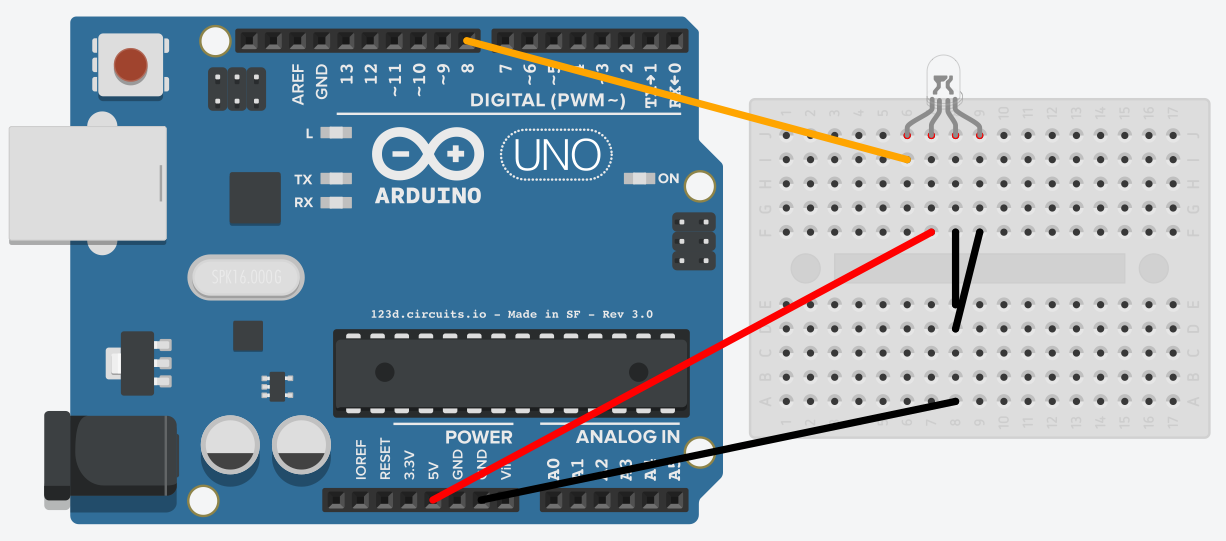
\includegraphics[width=\textwidth]{arduino-pir-wiring.png}
  \caption{The figure depicts wiring for a PIR motion sensor. A LED is shown in
    the figure, for a lack of a PIR component in the software generating the
    wiring schematics.}
  \label{fig:arduino_pir_wiring}
\end{figure}

\subsubsection{Sampling Input Data}

To reduce noise on the signal of the sensor, a simple statistical algorithm is
performed on the input data. The purpose of the algorithm is to increase reliability of the input data. Since the data can include false detection of objects that are not present, the algorithm is there to reduce  faulty data.  Essentially the data is reduced to two tiers
of data. First, the input data is accumulated into a tier1 low and a tier1 high
counter. When $n_{tier1}$ number of samples have been collected, a tier2 sampling round begins. If tier1
had more high counts than low counts, tier2 high is incremented and the opposite if
tier1 had the most lows. When the sample count of tier2 has reached a number
$n_{tier2}$, the calculated signal can be reported. If tier2 had the most highs,
report high and vice versa for tier2 lows.